%----------------------------------------------------------------------------------------
%    PACKAGES AND THEMES
%----------------------------------------------------------------------------------------
\documentclass[aspectratio=169,xcolor=dvipsnames]{beamer}
\makeatletter
\def\input@path{{../BeamerTemplate/theme/}}
\makeatother
\usetheme{CleanEasy}
\usepackage[utf8]{inputenc}
\usepackage{lmodern}
\usepackage[T1]{fontenc}
\usepackage{fix-cm}
\usepackage{amsmath}
\usepackage{mathtools}
\usepackage{listings}
\usepackage{xcolor}
\usepackage{hyperref}
\usepackage{graphicx}
\usepackage{booktabs}
\usepackage{tikz}
\usetikzlibrary{positioning, shapes, arrows, calc, decorations.pathreplacing, arrows.meta, backgrounds, patterns, overlay-beamer-styles}
\usepackage{etoolbox}
\usepackage{animate}

%----------------------------------------------------------------------------------------
%    LAYOUT CONFIGURATION
%----------------------------------------------------------------------------------------
\input{../BeamerTemplate/configs/configs}

%----------------------------------------------------------------------------------------
%    TITLE PAGE CONFIGURATION
%----------------------------------------------------------------------------------------
\title[Advanced Data Structures]{Data Structures: Advanced Data Structures}
\author{Minseok Jeon}
\institute{DGIST}
\date{\today}

% Simple title page without logos
\titlegraphic{}

%----------------------------------------------------------------------------------------

\begin{document}

\begin{frame}[plain]
  \titlepage
\end{frame}

\begin{frame}[plain]{Contents}
  \tableofcontents
\end{frame}

%----------------------------------------------------------------------------------------
%    INTRODUCTION
%----------------------------------------------------------------------------------------
\section{Introduction}

\begin{frame}{Advanced Data Structures}
  \begin{definition}
    \textbf{Advanced data structures} are specialized structures optimized for performance and specific problem domains.
  \end{definition}

  \vspace{0.5cm}

  \begin{block}{Knowledge Points}
    \begin{enumerate}
      \item Hash tables and hashing
      \item Collision handling: chaining/open addressing
      \item Tries (prefix trees)
      \item Disjoint Set / Union-Find
      \item Segment Trees and Fenwick Trees
      \item B-Trees and B+ Trees
      \item Real-world applications
    \end{enumerate}
  \end{block}
\end{frame}

%----------------------------------------------------------------------------------------
%    HASH TABLES
%----------------------------------------------------------------------------------------
\section{Hash Tables and Hashing}

\begin{frame}{What is a Hash Table?}
  \begin{definition}
    A \textbf{hash table} (hash map) provides O(1) average-case insertion, deletion, and lookup by mapping keys to values using a \textbf{hash function}.
  \end{definition}

  \vspace{0.3cm}

  \begin{columns}
    \begin{column}{0.5\textwidth}
      \textbf{Core Concept:}
      \begin{center}
        Key → Hash Function → Index → Value
      \end{center}

      \vspace{0.3cm}

      \begin{exampleblock}{Example}
        "apple" → hash("apple") = 5 → array[5] = 120
      \end{exampleblock}
    \end{column}
    \begin{column}{0.45\textwidth}
      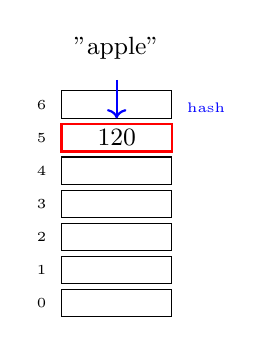
\begin{tikzpicture}[scale=0.7]
        % Array
        \foreach \i in {0,...,6} {
          \draw (0,\i*0.6) rectangle (2,\i*0.6+0.5);
          \node[left] at (-0.1,\i*0.6+0.25) {\tiny \i};
        }

        % Highlight index 5
        \draw[red, thick] (0,3) rectangle (2,3.5);
        \node at (1,3.25) {\small 120};

        % Arrow
        \node[above] at (1,4.5) {\small "apple"};
        \draw[->, thick, blue] (1,4.3) -- (1,3.6);
        \node[right, blue] at (2.1,3.8) {\tiny hash};
      \end{tikzpicture}
    \end{column}
  \end{columns}
\end{frame}

\begin{frame}{Good Hash Function Properties}
  \begin{columns}
    \begin{column}{0.48\textwidth}
      \begin{block}{Essential Properties}
        \begin{enumerate}
          \item \textbf{Deterministic}
          \begin{itemize}
            \item Same key always produces same hash
          \end{itemize}
          \item \textbf{Uniform distribution}
          \begin{itemize}
            \item Spreads keys evenly across table
          \end{itemize}
          \item \textbf{Fast to compute}
          \begin{itemize}
            \item O(1) time
          \end{itemize}
          \item \textbf{Minimize collisions}
          \begin{itemize}
            \item Different keys should have different hashes
          \end{itemize}
        \end{enumerate}
      \end{block}
    \end{column}
    \begin{column}{0.48\textwidth}
      \begin{block}{Common Hash Functions}
        \textbf{1. Division Method:}
        \begin{center}
          h(key) = key \% m
        \end{center}

        \vspace{0.2cm}

        \textbf{2. Multiplication Method:}
        \begin{center}
          h(key) = $\lfloor m \times (key \times A \bmod 1) \rfloor$
        \end{center}

        \vspace{0.2cm}

        \textbf{3. String Hashing:}
        \begin{center}
          Polynomial hash with prime base
        \end{center}
      \end{block}
    \end{column}
  \end{columns}
\end{frame}

\begin{frame}{Collisions and Load Factor}
  \begin{alertblock}{Problem: Collisions}
    When two different keys hash to the same index:
    \begin{center}
      hash("apple") = 5 \\
      hash("orange") = 5  \quad \textbf{← Collision!}
    \end{center}
  \end{alertblock}

  \vspace{0.3cm}

  \begin{columns}
    \begin{column}{0.48\textwidth}
      \begin{block}{Load Factor}
        Ratio of filled slots to total slots:
        \begin{center}
          $\alpha = \frac{n}{m}$
        \end{center}
        where n = number of elements \\
        m = table size

        \vspace{0.2cm}

        \textbf{Example:} 7 elements in table of size 10 \\
        → Load factor = 0.7
      \end{block}
    \end{column}
    \begin{column}{0.48\textwidth}
      \begin{block}{When to Resize}
        \begin{itemize}
          \item Typically resize when $\alpha$ > 0.7
          \item Double the table size
          \item Rehash all existing elements
          \item Maintains O(1) operations
        \end{itemize}
      \end{block}
    \end{column}
  \end{columns}
\end{frame}

\begin{frame}{Hash Table Complexity}
  \begin{table}
    \centering
    \begin{tabular}{l|c|c}
      \toprule
      \textbf{Operation} & \textbf{Average Case} & \textbf{Worst Case} \\
      \midrule
      Insert & O(1) & O(n) \\
      Delete & O(1) & O(n) \\
      Search & O(1) & O(n) \\
      Space & O(n) & O(n) \\
      \bottomrule
    \end{tabular}
  \end{table}

  \vspace{0.3cm}

  \begin{alertblock}{Note}
    Worst case occurs when all keys collide into the same slot. With a good hash function and proper load factor management, average case O(1) is achieved.
  \end{alertblock}

  \vspace{0.3cm}

  \begin{exampleblock}{Applications}
    Databases (indexing), caching, symbol tables (compilers), sets, counting frequencies, detecting duplicates
  \end{exampleblock}
\end{frame}

% %----------------------------------------------------------------------------------------
% %    COLLISION HANDLING
% %----------------------------------------------------------------------------------------
\section{Collision Handling}

\begin{frame}{Two Main Collision Resolution Strategies}
  \begin{columns}
    \begin{column}{0.48\textwidth}
      \begin{block}{1. Chaining (Separate Chaining)}
        \begin{itemize}
          \item Each slot contains a linked list
          \item Colliding elements form a chain
          \item Never fills up completely
        \end{itemize}

        \vspace{0.3cm}

        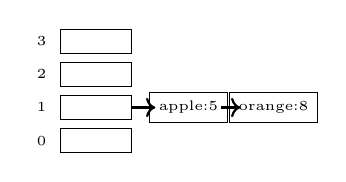
\begin{tikzpicture}[scale=0.6]
          \foreach \i in {0,1,2,3} {
            \draw (0,\i*0.7) rectangle (1.5,\i*0.7+0.5);
            \node[left] at (-0.1,\i*0.7+0.25) {\tiny \i};
          }

          % Chain at index 1
          \draw[thick,->] (1.5,0.95) -- (2,0.95);
          \node[draw] at (2.7,0.95) {\tiny apple:5};
          \draw[thick,->] (3.4,0.95) -- (3.8,0.95);
          \node[draw] at (4.5,0.95) {\tiny orange:8};
        \end{tikzpicture}
      \end{block}
    \end{column}
    \begin{column}{0.48\textwidth}
      \begin{block}{2. Open Addressing}
        \begin{itemize}
          \item All elements in table itself
          \item Probe for next empty slot
          \item Must maintain load factor < 1.0
        \end{itemize}

        \vspace{0.3cm}

        \textbf{Probing Methods:}
        \begin{itemize}
          \item Linear: h(k) + i
          \item Quadratic: h(k) + $i^2$
          \item Double hashing: $h_1$(k) + i*$h_2$(k)
        \end{itemize}
      \end{block}
    \end{column}
  \end{columns}
\end{frame}

\begin{frame}{Chaining Implementation}
  \begin{columns}
    \begin{column}{0.48\textwidth}
      \begin{block}{Advantages}
        \begin{itemize}
          \item $\checkmark$ Simple to implement
          \item $\checkmark$ Never fills up
          \item $\checkmark$ Good for unknown size
          \item $\checkmark$ Deletion is easy
        \end{itemize}
      \end{block}

      \begin{block}{Disadvantages}
        \begin{itemize}
          \item $\times$ Extra memory for pointers
          \item $\times$ Poor cache performance
          \item $\times$ Chains can become long
        \end{itemize}
      \end{block}
    \end{column}
    \begin{column}{0.48\textwidth}
      \begin{exampleblock}{Visual Example}
        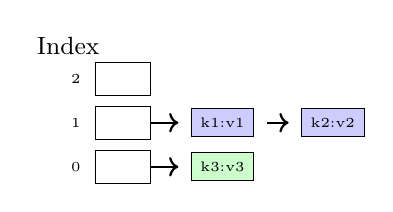
\begin{tikzpicture}[scale=0.7]
          % Table
          \node at (-0.5,2.5) {\small Index};
          \foreach \i in {0,1,2} {
            \draw (0,\i*0.8) rectangle (1,\i*0.8+0.6);
            \node[left] at (-0.1,\i*0.8+0.3) {\tiny \i};
          }

          % Chain 1
          \draw[thick,->] (1,1.1) -- (1.5,1.1);
          \node[draw,fill=blue!20] at (2.3,1.1) {\tiny k1:v1};
          \draw[thick,->] (3.1,1.1) -- (3.5,1.1);
          \node[draw,fill=blue!20] at (4.3,1.1) {\tiny k2:v2};

          % Single element
          \draw[thick,->] (1,0.3) -- (1.5,0.3);
          \node[draw,fill=green!20] at (2.3,0.3) {\tiny k3:v3};
        \end{tikzpicture}
      \end{exampleblock}
    \end{column}
  \end{columns}
\end{frame}

\begin{frame}{Open Addressing Strategies}
  \begin{block}{Linear Probing}
    Try consecutive slots: h(k), h(k)+1, h(k)+2, ...

    \textbf{Problem:} Primary clustering (keys cluster together)
  \end{block}

  \begin{block}{Quadratic Probing}
    Try quadratic intervals: h(k), h(k)+$1^2$, h(k)+$2^2$, h(k)+$3^2$, ...

    \textbf{Reduces} primary clustering but can cause secondary clustering
  \end{block}

  \begin{block}{Double Hashing}
    Use second hash function: h(k, i) = ($h_1$(k) + i * $h_2$(k)) \% m

    \textbf{Best} collision resolution for open addressing
  \end{block}

  \begin{alertblock}{Important}
    Must use tombstone markers for deletions to maintain probe sequences
  \end{alertblock}
\end{frame}

\begin{frame}{Chaining vs Open Addressing}
  \begin{table}
    \centering
    \small
    \begin{tabular}{l|p{4cm}|p{4cm}}
      \toprule
      \textbf{Feature} & \textbf{Chaining} & \textbf{Open Addressing} \\
      \midrule
      Memory & Extra (pointers) & More compact \\
      Cache performance & Poor & Better \\
      Load factor & Can exceed 1.0 & Must stay < 1.0 \\
      Deletion & Easy & Complex (tombstones) \\
      Implementation & Simple & More complex \\
      Best for & Unknown size & Known size, high performance \\
      \bottomrule
    \end{tabular}
  \end{table}

  \vspace{0.3cm}

  \begin{exampleblock}{Real-World}
    \textbf{Python's dict} uses open addressing with pseudo-random probing (optimized version of double hashing)
  \end{exampleblock}
\end{frame}

% %----------------------------------------------------------------------------------------
% %    TRIES
% %----------------------------------------------------------------------------------------
\section{Tries (Prefix Trees)}

\begin{frame}{What is a Trie?}
  \begin{definition}
    A \textbf{trie} (pronounced "try") is a tree-like structure for storing strings where each node represents a character. Excellent for prefix-based operations.
  \end{definition}

  \vspace{0.3cm}

  \begin{columns}
    \begin{column}{0.45\textwidth}
      \begin{block}{Storing: "cat", "car", "dog"}
        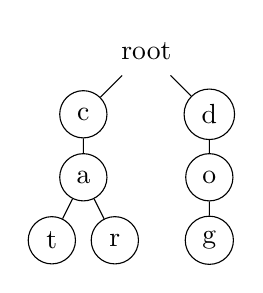
\begin{tikzpicture}[scale=0.8,
          every node/.style={circle, draw, minimum size=6mm}]
          \node[rectangle, draw=none] (root) at (0,0) {root};
          \node (c) at (-1,-1) {c};
          \node (d) at (1,-1) {d};
          \node (a) at (-1,-2) {a};
          \node (o) at (1,-2) {o};
          \node (t) at (-1.5,-3) {t};
          \node (r) at (-0.5,-3) {r};
          \node (g) at (1,-3) {g};

          \draw (root) -- (c);
          \draw (root) -- (d);
          \draw (c) -- (a);
          \draw (d) -- (o);
          \draw (a) -- (t);
          \draw (a) -- (r);
          \draw (o) -- (g);
        \end{tikzpicture}
      \end{block}
    \end{column}
    \begin{column}{0.5\textwidth}
      \begin{block}{Key Properties}
        \begin{itemize}
          \item Each path = a word
          \item Common prefixes share paths
          \item Fast prefix lookups
          \item Space-efficient for common prefixes
        \end{itemize}
      \end{block}

      \begin{exampleblock}{Operations}
        \begin{itemize}
          \item Insert: O(m)
          \item Search: O(m)
          \item Prefix search: O(m)
          \item Autocomplete: O(m + k)
        \end{itemize}
        where m = word length, k = results
      \end{exampleblock}
    \end{column}
  \end{columns}
\end{frame}

\begin{frame}{Trie Operations}
  \begin{columns}
    \begin{column}{0.48\textwidth}
      \begin{block}{Insert Word}
        \begin{enumerate}
          \item Start at root
          \item For each character:
          \begin{itemize}
            \item Create node if needed
            \item Move to child node
          \end{itemize}
          \item Mark end of word
        \end{enumerate}
      \end{block}

      \begin{block}{Search Word}
        \begin{enumerate}
          \item Start at root
          \item Follow characters
          \item Check end-of-word marker
        \end{enumerate}
      \end{block}
    \end{column}
    \begin{column}{0.48\textwidth}
      \begin{block}{Autocomplete}
        \begin{enumerate}
          \item Navigate to prefix end
          \item DFS from that node
          \item Collect all words in subtree
        \end{enumerate}
      \end{block}

      \begin{exampleblock}{Example}
        Prefix: "app" \\
        Results: \\
        - app \\
        - apple \\
        - application \\
        - apply
      \end{exampleblock}
    \end{column}
  \end{columns}
\end{frame}

\begin{frame}{Trie Applications}
  \begin{columns}
    \begin{column}{0.48\textwidth}
      \begin{block}{1. Autocomplete Systems}
        \begin{itemize}
          \item Google search suggestions
          \item IDE code completion
          \item Command-line completion
        \end{itemize}
      \end{block}

      \begin{block}{2. Spell Checking}
        \begin{itemize}
          \item Microsoft Word
          \item Browser spell check
          \item Find words within edit distance
        \end{itemize}
      \end{block}
    \end{column}
    \begin{column}{0.48\textwidth}
      \begin{block}{3. IP Routing}
        \begin{itemize}
          \item Longest prefix matching
          \item Network routing tables
        \end{itemize}
      \end{block}

      \begin{block}{4. Phone Contacts}
        \begin{itemize}
          \item T9 predictive text
          \item Contact search
        \end{itemize}
      \end{block}
    \end{column}
  \end{columns}

  \vspace{0.3cm}

  \begin{alertblock}{Trie vs Hash Table}
    Trie: O(m) exact search, O(m) prefix search, sorted order \\
    Hash Table: O(1) exact search, O(n) prefix search, no order
  \end{alertblock}
\end{frame}

% %----------------------------------------------------------------------------------------
% %    UNION-FIND
% %----------------------------------------------------------------------------------------
\section{Disjoint Set / Union-Find}

\begin{frame}{Disjoint Set (Union-Find)}
  \begin{definition}
    A data structure that efficiently handles partitioning of elements into disjoint (non-overlapping) sets.
  \end{definition}

  \vspace{0.3cm}

  \begin{columns}
    \begin{column}{0.48\textwidth}
      \begin{block}{Key Operations}
        \begin{itemize}
          \item \textbf{Find}: Which set does element belong to?
          \item \textbf{Union}: Merge two sets into one
          \item \textbf{Connected}: Are two elements in same set?
        \end{itemize}
      \end{block}

      \begin{exampleblock}{Example}
        Initial: \{0\}, \{1\}, \{2\}, \{3\}, \{4\} \\
        union(0, 1): \{0, 1\}, \{2\}, \{3\}, \{4\} \\
        union(2, 3): \{0, 1\}, \{2, 3\}, \{4\} \\
        union(0, 3): \{0, 1, 2, 3\}, \{4\}
      \end{exampleblock}
    \end{column}
    \begin{column}{0.48\textwidth}
      \begin{block}{Use Cases}
        \begin{itemize}
          \item Connected components in graphs
          \item Kruskal's MST algorithm
          \item Network connectivity
          \item Image processing (connected regions)
          \item Equivalence relations
        \end{itemize}
      \end{block}

      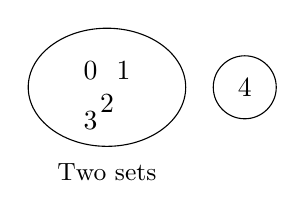
\begin{tikzpicture}[scale=0.7]
        % Set 1
        \node[draw, ellipse, minimum width=2cm, minimum height=1.5cm] at (0,0) {};
        \node at (-0.3,0.3) {0};
        \node at (0.3,0.3) {1};
        \node at (0,-0.3) {2};
        \node at (-0.3,-0.6) {3};

        % Set 2
        \node[draw, ellipse, minimum width=0.8cm, minimum height=0.8cm] at (2.5,0) {};
        \node at (2.5,0) {4};

        \node[below] at (0,-1.2) {\small Two sets};
      \end{tikzpicture}
    \end{column}
  \end{columns}
\end{frame}

\begin{frame}{Optimizations}
  \begin{columns}
    \begin{column}{0.48\textwidth}
      \begin{block}{1. Union by Rank}
        \begin{itemize}
          \item Track height of each tree
          \item Attach smaller tree under larger tree
          \item Keeps trees balanced
          \item Improves to O(log n)
        \end{itemize}

        \vspace{0.2cm}

        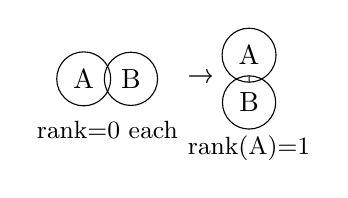
\begin{tikzpicture}[scale=0.6]
          \node[circle, draw] (a) at (0,0) {A};
          \node[circle, draw] (b) at (1,0) {B};
          \node[below] at (0.5,-0.7) {\small rank=0 each};

          \node at (2.5,0) {→};

          \node[circle, draw] (c) at (3.5,0.5) {A};
          \node[circle, draw] (d) at (3.5,-0.5) {B};
          \draw (c) -- (d);
          \node[below] at (3.5,-1) {\small rank(A)=1};
        \end{tikzpicture}
      \end{block}
    \end{column}
    \begin{column}{0.48\textwidth}
      \begin{block}{2. Path Compression}
        \begin{itemize}
          \item During find, point all nodes to root
          \item Flattens tree structure
          \item Future finds become faster
          \item Achieves O($\alpha$(n)) $\approx$ O(1)
        \end{itemize}

        \vspace{0.2cm}

        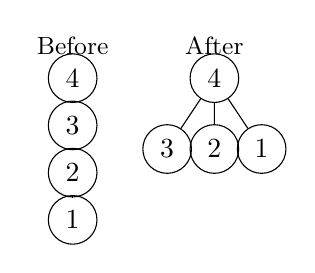
\begin{tikzpicture}[scale=0.6]
          % Before
          \node[circle, draw] (a) at (0,2) {4};
          \node[circle, draw] (b) at (0,1) {3};
          \node[circle, draw] (c) at (0,0) {2};
          \node[circle, draw] (d) at (0,-1) {1};
          \draw (a) -- (b) -- (c) -- (d);
          \node[above] at (0,2.3) {\small Before};

          % After
          \node[circle, draw] (e) at (3,2) {4};
          \node[circle, draw] (f) at (2,0.5) {3};
          \node[circle, draw] (g) at (3,0.5) {2};
          \node[circle, draw] (h) at (4,0.5) {1};
          \draw (e) -- (f);
          \draw (e) -- (g);
          \draw (e) -- (h);
          \node[above] at (3,2.3) {\small After};
        \end{tikzpicture}
      \end{block}
    \end{column}
  \end{columns}
\end{frame}

\begin{frame}{Union-Find Complexity}
  \begin{table}
    \centering
    \begin{tabular}{l|c|c}
      \toprule
      \textbf{Implementation} & \textbf{Find} & \textbf{Union} \\
      \midrule
      Naive & O(n) & O(n) \\
      Union by rank & O(log n) & O(log n) \\
      Path compression & O(log n) & O(log n) \\
      \textbf{Both optimizations} & \textbf{O($\alpha$(n)) $\approx$ O(1)} & \textbf{O($\alpha$(n)) $\approx$ O(1)} \\
      \bottomrule
    \end{tabular}
  \end{table}

  \vspace{0.3cm}

  \begin{alertblock}{$\alpha(n)$ - Inverse Ackermann Function}
    \begin{itemize}
      \item Grows \textbf{extremely slowly}
      \item $\alpha(n)$ < 5 for any practical n
      \item Essentially constant time in practice
    \end{itemize}
  \end{alertblock}

  \begin{exampleblock}{Application: Kruskal's MST}
    Sort edges: O(E log E), Process edges with Union-Find: O(E * $\alpha$(V)) $\approx$ O(E)
  \end{exampleblock}
\end{frame}

% %----------------------------------------------------------------------------------------
% %    SEGMENT TREES
% %----------------------------------------------------------------------------------------
\section{Segment Trees and Fenwick Trees}

\begin{frame}{Range Query Problem}
  \begin{block}{Problem}
    Given an array, efficiently answer queries like:
    \begin{itemize}
      \item Sum of elements in range [L, R]
      \item Minimum/maximum in range [L, R]
      \item Update single element
    \end{itemize}
  \end{block}

  \begin{alertblock}{Naive Approach}
    \begin{itemize}
      \item Range query: O(n) - iterate through range
      \item Update: O(1)
      \item Too slow for multiple queries!
    \end{itemize}
  \end{alertblock}

  \begin{exampleblock}{Goal}
    Both operations in O(log n) time
  \end{exampleblock}
\end{frame}

\begin{frame}{Segment Tree Structure}
  \begin{columns}
    \begin{column}{0.45\textwidth}
      \textbf{Array:} [1, 3, 5, 7, 9, 11]

      \vspace{0.3cm}

      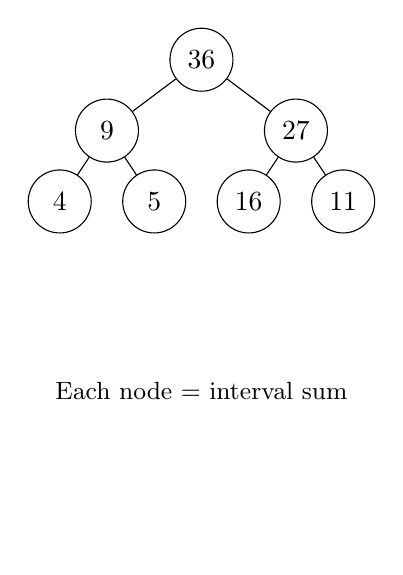
\begin{tikzpicture}[scale=0.6,
        every node/.style={circle, draw, minimum size=8mm}]
        \node (root) at (0,0) {36};
        \node (l1) at (-2,-1.5) {9};
        \node (r1) at (2,-1.5) {27};
        \node (l2) at (-3,-3) {4};
        \node (m2) at (-1,-3) {5};
        \node (r2) at (1,-3) {16};
        \node (rr2) at (3,-3) {11};

        \draw (root) -- (l1);
        \draw (root) -- (r1);
        \draw (l1) -- (l2);
        \draw (l1) -- (m2);
        \draw (r1) -- (r2);
        \draw (r1) -- (rr2);

        \node[draw=none, below] at (0,-3.7) {\small Each node = interval sum};
      \end{tikzpicture}
    \end{column}
    \begin{column}{0.5\textwidth}
      \begin{block}{Key Ideas}
        \begin{itemize}
          \item Binary tree structure
          \item Each node represents an interval
          \item Leaf = single array element
          \item Internal node = sum/min/max of children
          \item Height = O(log n)
        \end{itemize}
      \end{block}

      \begin{block}{Operations}
        \begin{itemize}
          \item Build: O(n)
          \item Query range: O(log n)
          \item Update element: O(log n)
        \end{itemize}
      \end{block}
    \end{column}
  \end{columns}
\end{frame}

\begin{frame}{Fenwick Tree (Binary Indexed Tree)}
  \begin{columns}
    \begin{column}{0.48\textwidth}
      \begin{block}{Advantages}
        \begin{itemize}
          \item More space-efficient than segment tree
          \item O(n) space vs O(4n) for segment tree
          \item Simpler implementation
          \item Efficient for prefix sums
        \end{itemize}
      \end{block}

      \begin{block}{Limitations}
        \begin{itemize}
          \item Only works for prefix sums
          \item Cannot do min/max queries
          \item No range updates
          \item Less versatile than segment tree
        \end{itemize}
      \end{block}
    \end{column}
    \begin{column}{0.48\textwidth}
      \begin{block}{Key Operations}
        \begin{itemize}
          \item Update: Add delta to element
          \item Prefix sum: Sum from 0 to index
          \item Range sum: prefix(R) - prefix(L-1)
        \end{itemize}
      \end{block}

      \begin{exampleblock}{Bit Trick}
        Uses bit manipulation for tree navigation:
        \begin{itemize}
          \item Next: index + (index \& -index)
          \item Parent: index - (index \& -index)
        \end{itemize}
      \end{exampleblock}
    \end{column}
  \end{columns}
\end{frame}

\begin{frame}{Segment Tree vs Fenwick Tree}
  \begin{table}
    \centering
    \begin{tabular}{l|c|c}
      \toprule
      \textbf{Feature} & \textbf{Segment Tree} & \textbf{Fenwick Tree} \\
      \midrule
      Space & O(4n) & O(n) \\
      Build & O(n) & O(n log n) \\
      Query & O(log n) & O(log n) \\
      Update & O(log n) & O(log n) \\
      Range update & Yes (lazy prop) & No \\
      Versatility & High & Limited \\
      Implementation & Complex & Simple \\
      \bottomrule
    \end{tabular}
  \end{table}

  \vspace{0.3cm}

  \begin{block}{When to Use}
    \textbf{Segment Tree:} Need min/max/GCD queries, range updates, multiple query types \\
    \textbf{Fenwick Tree:} Only prefix sums, simpler implementation, memory constrained
  \end{block}
\end{frame}

% %----------------------------------------------------------------------------------------
% %    B-TREES
% %----------------------------------------------------------------------------------------
\section{B-Trees and B+ Trees}

\begin{frame}{Why B-Trees?}
  \begin{alertblock}{Problem with BSTs for Disk Storage}
    \begin{itemize}
      \item Disk access is \textbf{very slow} (milliseconds vs nanoseconds for RAM)
      \item Want to minimize disk reads
      \item BSTs read one node at a time
      \item Need to read large blocks of data at once
    \end{itemize}
  \end{alertblock}

  \vspace{0.3cm}

  \begin{block}{B-Tree Solution}
    \begin{itemize}
      \item Each node can have \textbf{multiple keys} (not just one)
      \item Each node has \textbf{multiple children}
      \item All leaves at same level (perfectly balanced)
      \item Optimized for disk I/O
      \item One node = one disk block
    \end{itemize}
  \end{block}
\end{frame}

\begin{frame}{B-Tree Structure}
  \begin{block}{Properties}
    Given minimum degree t $\ge$ 2:
    \begin{itemize}
      \item Each node has at least t-1 keys (except root)
      \item Each node has at most 2t-1 keys
      \item Each internal node has at least t children
      \item Each internal node has at most 2t children
      \item All leaves at same depth
    \end{itemize}
  \end{block}

  \begin{exampleblock}{Example B-Tree (t=3)}
    \begin{center}
      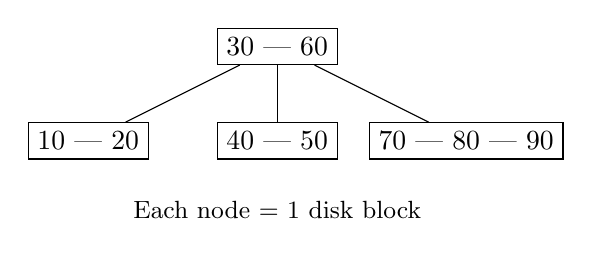
\begin{tikzpicture}[scale=0.8]
        \node[draw, rectangle] (root) at (0,0) {30 | 60};
        \node[draw, rectangle] (l) at (-3,-1.5) {10 | 20};
        \node[draw, rectangle] (m) at (0,-1.5) {40 | 50};
        \node[draw, rectangle] (r) at (3,-1.5) {70 | 80 | 90};

        \draw (root) -- (l);
        \draw (root) -- (m);
        \draw (root) -- (r);

        \node[below] at (0,-2.3) {\small Each node = 1 disk block};
      \end{tikzpicture}
    \end{center}
  \end{exampleblock}
\end{frame}

\begin{frame}{B+ Trees}
  \begin{columns}
    \begin{column}{0.48\textwidth}
      \begin{block}{Key Differences}
        \begin{enumerate}
          \item \textbf{All data in leaves}
          \begin{itemize}
            \item Internal nodes only store keys
          \end{itemize}
          \item \textbf{Leaves are linked}
          \begin{itemize}
            \item Sequential access
          \end{itemize}
          \item \textbf{Better for range queries}
          \begin{itemize}
            \item Traverse linked leaves
          \end{itemize}
        \end{enumerate}
      \end{block}
    \end{column}
    \begin{column}{0.48\textwidth}
      \begin{block}{Advantages}
        \begin{itemize}
          \item All leaves at same level
          \item Efficient range queries
          \item Internal nodes have more keys
          \item Less tree height
          \item Used in most databases
        \end{itemize}
      \end{block}

      \begin{exampleblock}{Used In}
        \begin{itemize}
          \item MySQL (InnoDB)
          \item PostgreSQL
          \item MongoDB
          \item File systems (HFS+, NTFS)
        \end{itemize}
      \end{exampleblock}
    \end{column}
  \end{columns}
\end{frame}

\begin{frame}{B-Tree Operations and Complexity}
  \begin{block}{Operations}
    \textbf{Search:}
    \begin{itemize}
      \item Find position in node (binary search within node)
      \item Follow child pointer if needed
      \item O(log n) disk reads
    \end{itemize}

    \textbf{Insert:}
    \begin{itemize}
      \item If node is full, split it
      \item Promote middle key to parent
      \item Recursively split if needed
      \item O(log n) disk reads/writes
    \end{itemize}
  \end{block}

  \begin{exampleblock}{Database Index Example}
    CREATE INDEX idx\_name ON users(name);

    Internally creates B+ tree where:
    \begin{itemize}
      \item Keys = user names (sorted)
      \item Values = pointers to table rows
      \item Fast lookup: O(log n) disk reads
    \end{itemize}
  \end{exampleblock}
\end{frame}

% %----------------------------------------------------------------------------------------
% %    APPLICATIONS
% %----------------------------------------------------------------------------------------
\section{Real-World Applications}

\begin{frame}{Hash Tables in Practice}
  \begin{columns}
    \begin{column}{0.48\textwidth}
      \begin{block}{Database Systems}
        \begin{itemize}
          \item Hash indexes for fast lookups
          \item Join operations
          \item Duplicate detection
        \end{itemize}
      \end{block}

      \begin{block}{Caching Systems}
        \begin{itemize}
          \item Redis
          \item Memcached
          \item Browser caches
          \item DNS caches
        \end{itemize}
      \end{block}
    \end{column}
    \begin{column}{0.48\textwidth}
      \begin{block}{Programming Languages}
        \begin{itemize}
          \item Python: dict
          \item Java: HashMap
          \item JavaScript: Object, Map
          \item C++: unordered\_map
        \end{itemize}
      \end{block}

      \begin{block}{Blockchain}
        \begin{itemize}
          \item Bitcoin transaction lookup
          \item Merkle tree verification
        \end{itemize}
      \end{block}
    \end{column}
  \end{columns}
\end{frame}

\begin{frame}{Tries in Practice}
  \begin{columns}
    \begin{column}{0.48\textwidth}
      \begin{block}{Search Engines}
        \begin{itemize}
          \item Google search suggestions
          \item Autocomplete
          \item Query correction
        \end{itemize}
      \end{block}

      \begin{block}{Text Editors}
        \begin{itemize}
          \item Microsoft Word spell check
          \item VSCode IntelliSense
          \item Vim command completion
        \end{itemize}
      \end{block}
    \end{column}
    \begin{column}{0.48\textwidth}
      \begin{block}{Networking}
        \begin{itemize}
          \item IP routing tables
          \item Longest prefix matching
          \item DNS resolution
        \end{itemize}
      \end{block}

      \begin{block}{Mobile Devices}
        \begin{itemize}
          \item T9 predictive text
          \item Contact search
          \item App name search
        \end{itemize}
      \end{block}
    \end{column}
  \end{columns}
\end{frame}

\begin{frame}{Union-Find in Practice}
  \begin{columns}
    \begin{column}{0.48\textwidth}
      \begin{block}{Network Analysis}
        \begin{itemize}
          \item Social network components
          \item Computer network connectivity
          \item Circuit connectivity
        \end{itemize}
      \end{block}

      \begin{block}{Image Processing}
        \begin{itemize}
          \item Connected region detection
          \item Image segmentation
          \item Blob detection
        \end{itemize}
      \end{block}
    \end{column}
    \begin{column}{0.48\textwidth}
      \begin{block}{Graph Algorithms}
        \begin{itemize}
          \item Kruskal's MST
          \item Cycle detection
          \item Dynamic connectivity
        \end{itemize}
      \end{block}

      \begin{block}{Other Applications}
        \begin{itemize}
          \item Compiler variable equivalence
          \item Percolation (physics)
          \item Maze generation
        \end{itemize}
      \end{block}
    \end{column}
  \end{columns}
\end{frame}

\begin{frame}{B-Trees in Practice}
  \begin{columns}
    \begin{column}{0.48\textwidth}
      \begin{block}{Database Systems}
        \begin{itemize}
          \item MySQL InnoDB storage engine
          \item PostgreSQL primary indexes
          \item MongoDB index structure
          \item SQLite database indexing
          \item Oracle Database
        \end{itemize}
      \end{block}

      \begin{block}{File Systems}
        \begin{itemize}
          \item HFS+ (macOS)
          \item NTFS (Windows)
          \item ext4 directory indexing
          \item ReiserFS
        \end{itemize}
      \end{block}
    \end{column}
    \begin{column}{0.48\textwidth}
      \begin{block}{Why B-Trees Win}
        \begin{enumerate}
          \item Minimize disk I/O
          \item Read large blocks at once
          \item Excellent for range queries
          \item Maintain sorted order
          \item Automatic balancing
        \end{enumerate}
      \end{block}

      \begin{alertblock}{Performance}
        For 1 million records with B-tree of degree 100:
        \begin{itemize}
          \item Height $\approx$ 3
          \item Search = 3 disk reads
          \item BST might need 20 reads!
        \end{itemize}
      \end{alertblock}
    \end{column}
  \end{columns}
\end{frame}

% %----------------------------------------------------------------------------------------
% %    SUMMARY
% %----------------------------------------------------------------------------------------
\section{Summary}

\begin{frame}{Key Takeaways - Part 1}
  \begin{block}{Hash Tables}
    \begin{itemize}
      \item O(1) average-case operations
      \item Chaining vs Open Addressing
      \item Load factor management crucial
      \item Powers dictionaries, caches, databases
    \end{itemize}
  \end{block}

  \begin{block}{Tries}
    \begin{itemize}
      \item Efficient prefix operations: O(m)
      \item Autocomplete, spell check, IP routing
      \item Space-efficient for common prefixes
      \item Trade memory for prefix speed
    \end{itemize}
  \end{block}
\end{frame}

\begin{frame}{Key Takeaways - Part 2}
  \begin{block}{Union-Find}
    \begin{itemize}
      \item Manages disjoint sets efficiently
      \item With optimizations: O($\alpha$(n)) $\approx$ O(1)
      \item Kruskal's MST, connectivity, image processing
      \item Union by rank + path compression essential
    \end{itemize}
  \end{block}

  \begin{block}{Segment Trees \& Fenwick Trees}
    \begin{itemize}
      \item Efficient range queries: O(log n)
      \item Segment tree: Versatile, complex
      \item Fenwick tree: Simple, limited to sums
      \item Applications: Range queries, inversions
    \end{itemize}
  \end{block}
\end{frame}

\begin{frame}{Key Takeaways - Part 3}
  \begin{block}{B-Trees \& B+ Trees}
    \begin{itemize}
      \item Optimized for disk storage
      \item Minimize disk I/O: O(log n) reads
      \item B+ Trees: Better for range queries
      \item Foundation of modern databases
    \end{itemize}
  \end{block}

  \vspace{0.3cm}

  \begin{alertblock}{Choosing the Right Structure}
    \begin{itemize}
      \item Consider access patterns
      \item Memory vs speed trade-offs
      \item Exact lookups $\to$ Hash table
      \item Prefix operations $\to$ Trie
      \item Range queries $\to$ Segment/Fenwick tree
      \item Disk storage $\to$ B-tree
      \item Dynamic connectivity $\to$ Union-Find
    \end{itemize}
  \end{alertblock}
\end{frame}

\begin{frame}{Complexity Comparison}
  \begin{table}
    \centering
    \footnotesize
    \begin{tabular}{l|c|c|c}
      \toprule
      \textbf{Data Structure} & \textbf{Key Operation} & \textbf{Time} & \textbf{Best For} \\
      \midrule
      Hash Table & Insert/Search/Delete & O(1) avg & Exact lookups \\
      Trie & Prefix search & O(m) & Prefix operations \\
      Union-Find & Union/Find & O($\alpha$(n)) & Connectivity \\
      Segment Tree & Range query & O(log n) & Range queries \\
      Fenwick Tree & Prefix sum & O(log n) & Sum queries \\
      B-Tree & Disk search & O(log n) & Disk storage \\
      \bottomrule
    \end{tabular}
  \end{table}

  \vspace{0.3cm}

  \begin{exampleblock}{Remember}
    No single data structure is best for everything. Choose based on your specific requirements and constraints.
  \end{exampleblock}
\end{frame}

\begin{frame}[plain]
  \begin{center}
    {\Huge Thank You!}

    \vspace{1cm}

    {\large Questions?}
  \end{center}
\end{frame}

\end{document}
